\documentclass[../projekt.tex]{subfiles}
\begin{document}
\graphicspath{ {images/} }

\chapter{Teoretický úvod} \label{teoreticky-uvod}

V~rámci řešení projektu musíme vyřešit dva základní problémy a to detekci aktivních hostů a následnou detekci otevřených portů.

V~této kapitole se podíváme na to jakým způsobem jsme vyřešili detekci aktivních hostů na přímo nebo nepřímo připojené síti. Zároveň se podíváme na způsob detekce otevřených portů TCP a UDP portů na zařízeních. 

\section{Detekce aktivních hostů}
V~rámci našeho programu máme detekovat aktivní hosty na síti. Dále máme specifikováno v~zadání\cite{Zadani}, že na přímo připojené síti máme detekovat všechna připojená zařízení a na nepřímo připojené síti detekovat zařízení respektovat RFC 1122\cite{RFC1122}.

V RFC 1122\cite{RFC1122} v~sekci 3.2.2.6 je definováno, že každý host na síti musí implementovat ICMP server, který, pokud mu dojde ICMP echo request zpráva, odpoví zprávou typu ICMP Echo reply. Tím pádem všichni hosté respektující RFC 1122 musí odpovídat na tyto zprávy. Pro skenování nepřímo připojené síti proto zvolíme použití ICMP echo zpráv.

V přímo připojené síti je potřeba detekovat všechna zařízení. ICMP protokol je pro toto řešení nevhodný, protože zařízení nemusí na ICMP zprávy odpovídat (viz \cite{ICMP_Dsiable}). Z~tohoto důvodu budeme pro detekci v~přímo připojené síti používat Address Resolution Protocol, jehož blokování by znemožnilo zařízení síťovou komunikaci.

\subsection{Internet Control Message Protocol (ICMP)} \label{icmp}
Internet Control Message Protocol je L3 protokol definovaný v~RFC 792\cite{RFC0792}. Tento protokol byl navržen pro detekci chyb, řešení problémů na síti a detekci nedostupnosti zařízení. Seznam všech typů naleznete v~již zmiňovaném RFC\cite{RFC0792}.

\begin{figure}
    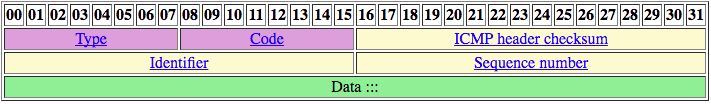
\includegraphics[width=0.8\textwidth]{IcmpHeader}
    \centering
    \caption{Tvar hlavičky pro ICMP Echo request/reply}
\end{figure}

Nás konkrétně zajímají zprávy typu Echo Request a Echo Reply. Jakmile je na hosta zaslána zpráva zpráva typu Echo Request. Tento host (za předpokladu, že dodržuje RFC 1122\cite{RFC1122}) na tuto zprávu odpoví zprávou typu Echo Reply se stejnými daty jako byly v~původní zprávě (tato data mohou být použita odesilatelem requestu pro kontrolu správnosti odpovědi).

\subsection{Address Resolution Protocol (ARP)} \label{arp}
Address Resolution Protocol je L3 protokol definovaný v~RFC 826\cite{RFC0826}. Tento protokol je navržený pro překlad L2 adres (v našem případě MAC adresa) na L3 adresy (v našem případě IPv4 adresa).

ARP paket obsahuje informace o:
\begin{itemize}
    \item typu zařízení
    \item typu L3 protokolu jehož adresu potřebujeme (v našem případě IPv4)
    \item velikosti hardwareové (L2) adresy
    \item velikosti adresy používané požadovaným L4 protokolem
    \item L2 a L3 adresa odesilatele
    \item L2 (broadcast) a L3 adresa, kterou hledáme
\end{itemize}

Odesilatel nejprve pošle na L2 broadcast dotaz, kdo má danou L3 adresu. Pokud je na síti připojen příjemce, tak na zprávu odpoví tentokrát už na unicast L2 adresy odesilatele, že on je ten hledaný a má tuto L3 adresu.

\section{Zjišťování otevřených portů}

V případě zjišťování, které porty jsou otevřené, musíme rozlišovat transportní protokoly, který služba běžící na daném využívá pro přenos dat. Výrazně se liší, jakým způsobem funguje zjišťování otevřených portů služeb používajícíh TCP, které vytváří spojení, a služeb používajících UDP, které je bezstavové.

\subsection{Transmission Control Protocol (TCP)} \label{tcp}

Transmission Control Protocol je L4 protokol definovaný v~RFC 793\cite{RFC0793}. Tento protokol je používaný pro spolehlivý a bezchybný přenos dat přes síť.

Při navázání spojení TCP dochází pomocí techniky zvané threeway handshake. Navázání spojení vypadá takto:
\begin{enumerate}
    \item Klient odešle na server TCP paket s~nastaveným příznakem SYN, náhodným číslem sekvence a potvrzovacím číslem 0.
    \item Server paket přijme a odpoví a odešle klientovi paket s~nastavenými příznaky SYN a ACK, zvýšeným potvrzovacím číslem rovným klientovu číslu sekvence + 1 a vlastním náhodným číslem sekvence.
    \item Klient odešle na server paket s~příznakem ACK a potvrzovacím číslem rovným serverovému číslu sekvence 1 větší a vlastním číslem sekvence zvětšeným rovněž 0 1.
\end{enumerate} 

Při skenování portů můžeme právě tohoto využít. Pokud pošleme na všechny porty paket s~nastaveným příznakem SYN, tak by nám ze všech otevřených portů měla přijít odpověď s~nastavenými SYN a ACK příznaky. V~případě, že bude port zavřený měla by nám přijít zpráva s~nastavenými příznaky RST a ACK. 

Důležité je v~případě, že jsme se dozvěděli, že je port otevřený zaslat klientovi požadavek s~příznakem RST a ukončit tak připojení, aby nezůstávalo na druhé straně napůl otevřené připojení.

\subsection{User Datagram Protocol (UDP)} \label{udp}

User Datagram Protocol je L4 protokol definovaný v~RFC 768\cite{RFC0768}. UDP je nespojovaný transportní protokol s~minimálním množstvím režie. Pakety posílané pomocí UDP nemají žádnou jistotu jejich pořadí, doručení nebo duplikace. 

Vzhledem k~tomu, že je protokol nespojovaný, nelze u~něj provádět detekci otevřených portů jako u~TCP (více v~kapitole \ref{tcp}). UDP díky svému nespojovanému chování neposkytuje žádný způsob detekce zda paket došel z~klienta na server. V~tomto nám pomáhá ICMP, které jsme tu zmínili v~předchozí kapitole. V~případě, že pošleme UDP paket na server, nám server odpoví ICMP zprávou typu Destination Unreachable, díky které jsme schopni říct, že port je uzavřen. V~případě, že nám ICMP zpráva nepřijde je port považován za otevřený.



\end{document}